The structure of the classes in the project have been dictated by how the json code from a search on the Spotify Web API is structured. When using the Web API to search on Spotify three different items can be found Track, Album and Artist. For each search it must be specified what item that is being searched for. To minimize the requirements for the user it was decided that the user should not specify what item he or she is searching for but rather he or she should write the search string and get a complete list of the results for all items represented. Therefore it has been implemented that it is possible, when creating a Search object, to specify from an enum which of the three items or all three are being searched for. When choosing all three, which is what we do for the users, three idividual searches are created and the results are represented in a complete structure shown in \cref{fig:WebAPIUML}.

\begin{figure}
  \centering
  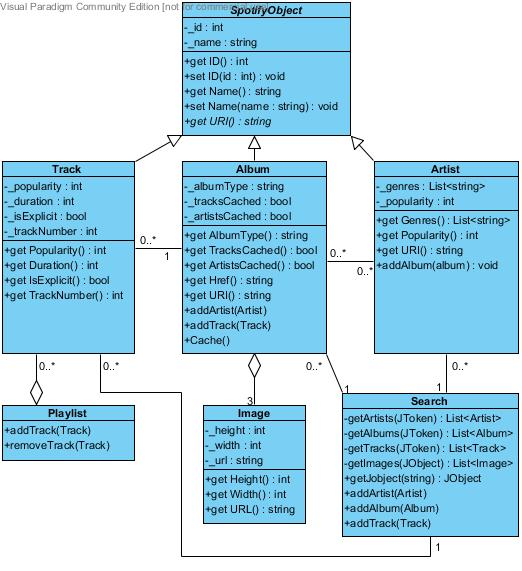
\includegraphics[width=0.5\linewidth]{Images/WebAPIUML.jpg}
  \caption{A class diagram showing the class structure of the results generated from a search}
  \label{fig:WebAPIUML}
\end{figure}